% !TeX spellcheck = ru_RU
%pdflatex, utf8
\documentclass[unicode, 10pt, a5paper, oneside]{article}

% Установка полей страницы
%\usepackage{anysize}
%\marginsize{0.3cm}{0.3cm}{0.3cm}{0.3cm}
\usepackage[a5paper, margin=0.3cm, bindingoffset=0cm]{geometry}

% Поддержка русского языка
\usepackage[T2A]{fontenc}		% Корректная кодировка шрифта при использовании cm-super
\usepackage[utf8]{inputenc}		% Кодировка ввода
\usepackage[russian]{babel}		% Словарь расстановки переносов
%\usepackage{cmap}				% Перекодировка символов в pdf при использовании обычного cm

% Всякие математические фишки
\usepackage{amsmath}
\usepackage{amsfonts}
\usepackage{amssymb}

% Изменение цвета, работа с графикой
\usepackage{color}
\usepackage[pdftex]{graphicx}
\graphicspath{{images/}}

% Команда для вставки ссылок \url{URL}
\usepackage[hyphens]{url}
\urlstyle{rm}					% Стиль шрифта ссылок: с засечками

% Кликабельные ссылки внутри документа
\usepackage[unicode]{hyperref}

% Включает отступ у первого абзаца в разделе
\usepackage{indentfirst}

% Настрйока стиля списков
\usepackage{enumitem}
\setlist{noitemsep, leftmargin=*, labelindent=\parindent, topsep=0pt, parsep=0pt, partopsep=0pt}

\setlist[itemize,1]{label=$\diamond$}
\setlist[itemize,2]{label=\textendash}
\setlist[itemize,3]{label=$\star$}

\renewcommand{\alph}[1]{\asbuk{#1}} % Костыль для кирилической нумерации вместо латинской
\setlist[enumerate,1]{label=\arabic*)}
\setlist[enumerate,2]{label=\alph*)}
\setlist[enumerate,3]{label=(\arabic*)}


\usepackage{textcomp}			% Команды для вставки разных символов (градусы, проценты, итд)
\usepackage{float}				% Размещение плавающих объектов там где они созданы (X)
\usepackage{wrapfig}			% Обтекаемые текстом рисунки

% Подписи у флоатов
\setlength{\intextsep}{0pt} % Отстут вокруг плавающих окружений
\usepackage{caption}
\captionsetup{parskip=0pt}
\captionsetup[figure]{labelsep=period,justification=centering,singlelinecheck=false,textfont=small,labelfont=small,aboveskip=2pt,belowskip=0pt}

% Изменение формата заголовков разделов
\usepackage{titlesec}
\titleformat{\section}{\newpage\small\bfseries}{\thesection. }{0pt}{}{}
\titlespacing*{\section}{0pt}{0pt}{0pt}

\titleformat{\subsection}{\small\bfseries}{\thesubsection. }{0pt}{}{}
\titlespacing*{\subsection}{0pt}{0pt}{0pt}

\usepackage{array}				% Позволяет объявить свои типы колонок
\usepackage{calc}				% Математика, исп-ся для расчёта ширины колонки
\usepackage{longtable}			% Длинные таблицы

% Минимальный отступ в таблицах
\setlength{\tabcolsep}{1.5mm}

% Новые типы колонок. Ширина задётся как доля от linewidth
\newcolumntype{L}[1]{p{#1\linewidth-2\tabcolsep-2\arrayrulewidth}}
\newcolumntype{C}[1]{>{\centering}p{#1\linewidth-2\tabcolsep-2\arrayrulewidth}}
\newcolumntype{R}[1]{>{\raggedleft}p{#1\linewidth-2\tabcolsep-2\arrayrulewidth}}
\newcolumntype{U}[2]{p{#1\linewidth-(#2)}}

% Стараться не оставлять одиноких строк в начале и конце абзаца
\clubpenalty=1000
\widowpenalty=1000

% Расстановка отступов и переносов
\emergencystretch=2.5em			% Максимальный промежуток между словами
\tolerance=2000
\frenchspacing


\begin{document}

\setcounter{section}{150}

% Вопрос 151 ----------------------------------------------------------
\section{Системы хранения данных. Назначение. Три основные структуры систем хранения данных.}

С ростом производительности ЭВМ и увеличением объемов хранимой информации возникает необходимость в специальных внешних устройствах для хранения данных. ВЗУ большого объема обычно строятся на основе ленточных накопителей, которые обладают большим временем доступа и быстрым старением. Возникает задача хранения больших объемов данных с быстрым временем доступа.

Причинами появления СХД считают следующие: децентрализация хранения информации (организациям со временем приходится задействовать оборудование филиалов для хранения информации), низкий уровень защиты данных, низкая степень конфиденциальности передаваемых данных, требования к масштабируемости (неизвестно какие объемы информации потребуется хранить через несколько лет). Возникает необходимость в некой автоматизированной системе, которая хранила бы данные.

В простейшем случае структуру такой системы можно представить в следующем виде: \mbox{SCSI --- RAID-контроллер --- HDD (несколько)}.

К SCSI подключается RAID-контроллер с буферным каналом ввода/вывода и кэш-памятью достаточно большого объема. Задача RAID- контроллера обеспечить формирование RAID- массива: присваивание файлам своих адресов. Связь контроллера с HDD осуществляется по параллельным линиям с электрическими или оптическими сигналами.

За счет кэш-памяти RAID-контроллер обеспечивает высокую скорость доступа к данным, при этом задача буферного блока скомпоновать общий файл при нескольких запросах. Кроме того, в буферном блоке производится контроль информации, при необходимости с восстановлением.

Такие СХД подключаются к типовым интерфейсам, прежде всего к SCSI (до 640 Мб/с). Помимо него часто используется Fibre Channel --- интерфейс с оптическими линиями связи способный обеспечивать до 4 Гб/с.

\subsection*{Структура СХД}

Для подключения внешних дисков требуется внешний контроллер с высоким быстродействием, чтобы обеспечить приемлемую скорость передачи массива. Передача идет файлам не непрерывно, с попеременными чтением и записью, поэтому в структуру СХД должны входить следующие блоки:

\begin{figure}[H]
\centering
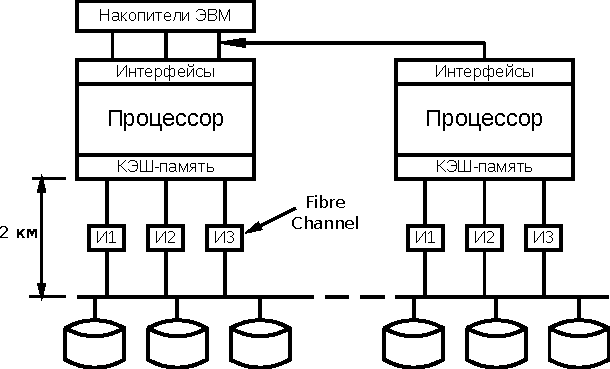
\includegraphics[width=0.6\textwidth]{151_struct.pdf}
\caption{Структура СХД}
\end{figure}

Процессор контроллера должен обладать высокой переключающей способностью, а интерфейс к ЭВМ должен позволять пересылать большие массивы данных. Связь со стойками с дисками невозможна без буферной памяти.

Информацию при передаче данных можно восстановить, но сбой при записи может привести к потере данных, поэтому система резервируется. Одновременно работают два контроллера, но доступ отдан одному. В случае возникновения ошибки, второй контроллер вступает в работу, его кэш-память так же страхует возможные потери информации.

Такие структуры входят в состав стоек, и часто не одна система хранения данных, а несколько, как бы отдельных.

\subsection*{Организация СХД}

В зависимости от объемов хранимой информации, сложности системы и требований к надежности можно выделить три основные структуры СХД:

\textit{Прямое включение <<DAS>>}. Сервер сети и сервер СХД разделены. Имеется толь одна линия доступа к СХД, что снижает надежность в случае отказа и скорость доступа к данным.

\begin{figure}[H]
\centering
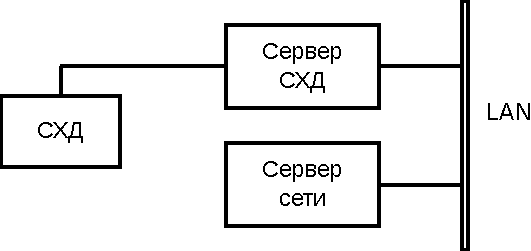
\includegraphics[width=0.4\textwidth]{151_das.pdf}
\caption{Прямое включение <<DAS>>}
\end{figure}

\textit{Прямое подключение в сеть <<NAS>>}. СХД является абонентом сети, обеспечивающим файловый доступ, и должна иметь соответствующее сетевое оборудование. У каждой стойки может быть свое особенное ПО.

\begin{figure}[H]
\centering
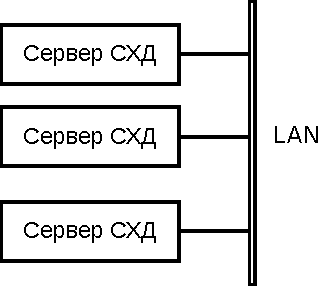
\includegraphics[width=0.25\textwidth]{151_nas.pdf}
\caption{Прямое подключение в сеть <<NAS>>}
\end{figure}

\textit{Сетевое подключение <<SAN>>}. Имеется возможность переключения каналов передачи информации. СХД подключается сразу к 2 каналам и, если один из них загружен, то используется второй. Система централизованная, но сложная и дорогая.

\begin{figure}[H]
\centering
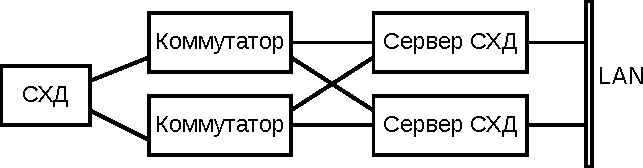
\includegraphics[width=0.6\textwidth]{151_san.pdf}
\caption{Сетевое подключение <<SAN>>}
\end{figure}


% Вопрос 152 ----------------------------------------------------------
\section{Основные понятия информационно-вычислительных систем, классификация по критерию потоков информации.}

Понятие вычислительная машина обычно применяют к вычислительному устройству, имеющему небольшие габариты и единую конструкцию. Обычно это устройство включает минимально необходимые функциональные узлы. Система относится к более сложным устройствам и объединяет функциональные блоки территориально разнесенные, чаще однотипные. В составе системы может быть несколько функциональных однотипных блоков. Понятие комплекс выше системы, его применяют к устройствам занимающим определенное пространство, т.е. разнесенные, имеющие каналы связи и разнотипные повторяющиеся функциональные блоки. Поскольку между комплексом и системой граница размыта, обычно их разделяют по конструктивному признаку. \textbf{Комплекс} --- это множество самостоятельных конструктивно устройств. \textbf{Сети} --- территориально разнесенные вычислительные устройства, использующие стандартные способы связи между собой.

Как правило, информационно- вычислительная система (ИВС) или информационно- вычислительный комплекс (ИВК) имеют прикладное назначение. Те или иные конфигурации предназначены для сбора и обработки информации, управления, диагностирования, автоматизированных рабочих мест. В этих структурах непосредственно вычислительные процедуры занимают не основную роль. Основным становится передача, хранение информации. В зависимости от состава системы изменяется конфигурация, динамические характеристики, надежность устройств. В процессе эволюции системы прошли длинный путь, поэтому появились различные конфигурации вычислительных систем.

\textbf{Классификация по потокам информации (по Флину)}

В любой ВС можно выделить два основных информационных потока: поток команд и поток данных, поэтому представляется 4 основных конфигурации:

\begin{enumerate}
\item ОКОД. Один поток команд, один поток данных.

Один процессор с раздельными памятью команд и данных. Это последовательная структура, в которой данные связаны с одной конкретной командой. Если необходимы новые данные, формируется новая команда или повторяется.

\begin{figure}[H]
\centering

\includegraphics[width=0.45\textwidth]{152_okod.pdf}
\caption{Организация ВС: один поток команд, один поток данных}
\end{figure}

\item ОКМД. Один поток команд, множество потоков данных.
\par Специализированные микропроцессоры использующиеся для параллельной обработки различных данных по одной команде. Эта структура наиболее близка к термину параллельная обработка, поскольку в каждый момент времени множество операндов преобразуются под управлением одинаковых команд. Параллельные системы с такой структурой применяют для обработки многомерной графики, сигналов от реальных датчиков, работающих в реальном времени.

\begin{figure}[H]
\centering
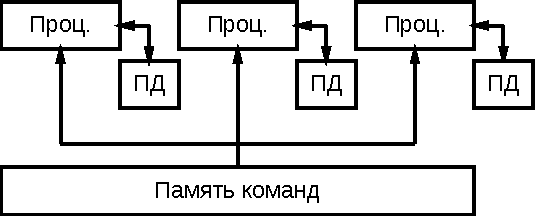
\includegraphics[width=0.45\textwidth]{152_okmd.pdf}
\caption{Организация ВС: один поток команд, множество потоков данных}
\end{figure}

\item МКОД. Множество потоков команд, один поток данных.
\par Конвейерная структура реализованная непосредственно на кристалле. Процессоры соединены в цепочку по шинам данных, при этом шины команд у каждого самостоятельные. В каждый момент времени выполняются разные команды в процессорах над одним потоком данных. Поток данных в этом случае --- последовательность операндов несущих информацию о какой-то величине. При этом каждое значение операнда последовательно преобразуется согласно поступающим командам.

\begin{figure}[H]
\centering
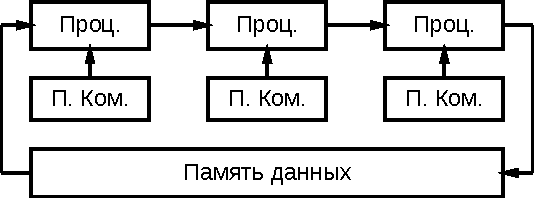
\includegraphics[width=0.45\textwidth]{152_mkod.pdf}
\caption{Организация ВС: множество потоков команд, один поток данных}
\end{figure}

\item МКМД. Множество потоков команд, множество потоков данных.
\par Матричная регулярная структура, где матрица процессоров в одном слое использует параллельную обработку, а последовательно по слоям --- конвейер. Такие структуры известны как однородные вычислительные системы. Применяются в сверхбыстродействующих специализированных системах работы с реальными сигналами.

\begin{figure}[H]
\centering
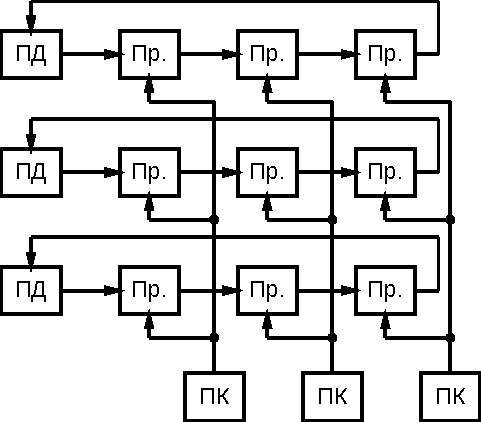
\includegraphics[width=0.45\textwidth]{152_mkmd.pdf}
\caption{Организация ВС: множество потоков команд, множество потоков данных}
\end{figure}

\end{enumerate}


% Вопрос 153 ----------------------------------------------------------
\section{Совмещение операций и многопрограммная работа. Режим работы в реальном времени.}

Режим работы ЭВМ --- это порядок прохождения задач (заданий) через ЭВМ. Задача --- это программа и данные, загруженные в ОП, т.е. программа вместе с выделенными ей ресурсами. Различают режимы работы двух типов --- однозадачный (однопрограммный) и мультизадачный (мультипрограммный).

В \textit{однопрограммном режиме} аппаратура ЭВМ выполняет одну пользовательскую программу под управлением и с использованием программ ОС. Практически это двухпрограммный режим: пользовательская программа плюс программа ОС. Но поскольку программы ОС являются сервисными, обслуживающими запросы пользователя, такой режим называют однопрограммным (однозадачным).

\begin{figure}[H]
\centering
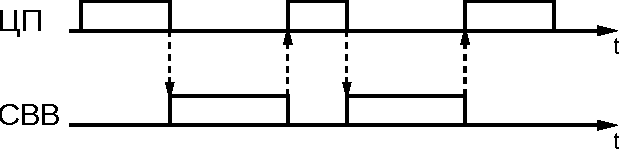
\includegraphics[width=0.5\textwidth]{153_single.pdf}
\caption{Диаграмма загруженности ЭВМ в однопрограммном режиме}
\end{figure}

Основное \textit{достоинство однопрограммного режима} --- минимальное время ответа на запросы пользователя. Все ресурсы ЭВМ (и аппаратные, и программные) находятся в распоряжении пользователя --- нет конкуренции за ресурсы. Пользователь монопольно владеет всеми ресурсами.

Основной \textit{недостаток однопрограммного режима} --- неэффективное использование оборудования, в частности, процессора: как видно из временной диаграммы, большую часть времени процессор простаивает.  Быстродействие системы ввода/вывода, обычно существенно ниже быстродействия процессора и памяти.

Как вариация однопрограммного режима существует \textit{пакетный режим}: в этом режиме пользователь подготавливает последовательность (пакет) запускаемых по очереди программ, что исключает ожидание ввода пользователя для запуска каждой последующей программы. Это несколько повышает реальную производительность системы.

В более мощных, дорогих ЭВМ с целью повышения эффективности использования оборудования применяется \textit{мультипрограммный режим}. В этом режиме, кроме программ ОС, в ОП компьютера располагаются и (по очереди) выполняются несколько (в общем случае М) программ пользователей, при этом, пока одна из программ ожидает завершения операций ввода/вывода, управление передаётся другой программе. Цель --- увеличение загрузки ЦП и, как следствие, производительности ЭВМ.

\begin{figure}[H]
\centering
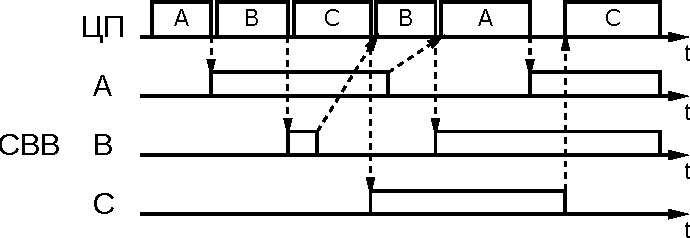
\includegraphics[width=0.6\textwidth]{153_multi.pdf}
\caption{Диаграмма загруженности ЭВМ в многопрограммном режиме}
\end{figure}

Мультипрограммный режим сложнее однопрограммного, поэтому к ВС предъявляет специальные требования. Для их реализации в состав ЭВМ вводятся специальные средства, которые и принято называть средствами мультипрограммирования. Средства, обеспечивающие заданный режим мультипрограммирования --- это управляющие программы ОС. Они обеспечивают требуемый порядок прохождения задач через ЭВМ, образуют основную часть --- ядро ОС.

\textit{Режим реального времени} применяют в вычислительных системах, работающих с физическими сигналами --- информационно-контролирующими, управляющими, обрабатывающими программами. Понятие это условно, поскольку время изменяется. Условие реального времени $ t_\text{обр.} < t_\text{пер.след.вх.сигн.}$. В этом режиме в первую очередь требуется быстрое измерение сигнала и занесение его в память, поэтому время начала работы процессора определяется временем поступления входного сигнала. Программа запускается по какому-то внешнему событию (чаще прерыванию).


% Вопрос 154 ----------------------------------------------------------
\section{Типы структур многопроцессорных ВС. Параллельные ЭВМ, классификация. Три архитектурных класса машин.}

Существует следующие типы структур многопроцессорных вычислительных машин:

\begin{itemize}
\item Векторно-конвеерные суперкомпьюетры
\item Симметричные мультипроцессорные системы (SMP)
\item Cистемы с массовым параллелизмом (MPP)
\item Кластерные системы
\end{itemize} 

Различают несколько классификаций параллельных ЭВМ:

\begin{itemize}
\item Классификация по Флинну (по потокам данных/команд)
	\begin{itemize}
	\item одиночный поток команд/одиночный поток данных (ОКОД)
	\item одиночный поток команд/множественный поток данных (ОКМД)
	\item множественный поток команд/одиночный поток данных (МКОД)
	\item множественный поток команд/множественный поток данных (МКМД)
	\end{itemize}
\item Классификация по программной организации
		\begin{itemize}
		\item с логическим программным управлением
		\item с управлением потоками данных
		\item с редукционно-программным упралением
		\end{itemize}
\item Классификация по архитектуре
\end{itemize} 

Существует три архитектурных класса машин:

\begin{itemize}
\item Централизованные машины (управление) --- один процессор, соединенный с памятью, единственная текущая команда передает управление единственной следующей команде
\item Машины с коммутацией пакетов --- конвейерный принцип, когда ряд процессоров, средства связи и память объединяются в последовательную структуру для решения текущей задачи.
\item Машины с обработкой выражений --- формируется набор из процессора, памяти, средств связи. Этот набор формируется как регулярная структура. Программа здесь достаточно большая по составу, в активном состоянии пребывают лишь некоторые составляющие, остальные находятся в состоянии ожидании.
\end{itemize}

% Вопрос 155 ----------------------------------------------------------
\section{Принципы ввода-вывода информации в ПЭВМ. Роль и структура контроллера ввода информации.}

Функционирование любого вычислителя складывается из процедур передачи информации между его отдельными функциональными блоками. При этом передача информации между внутренними РОН называется \textit{пересылка}, между процессором и памятью \textit{чтение/запись}, а между памятью и внешними устройствами \textit{ввод/вывод} информации. Наиболее продолжительными по времени процедурами считают операции ввода/вывода, поскольку внешние устройства в большинстве случаев имеют меньшее быстродействие, чем процессор или память, поэтому большое внимание на возможные варианты пересылки информации, рассматривая их с точки зрения снижения времени всей процедуры.

Доступ к внешним устройствам в большинстве случаев адресный, т. е. по структуре ввод/вывод не должен отличаться от чтения/записи. Но объем памяти значителен, значительна и шина адреса (минимум 16 разрядов). В тоже время число внешних устройств не может быть физически большим. В вычислителях системы DEC, i360 было принято ограничение на число внешних устройств 255. Это связано с байтом, хотя реально их значительно меньше. Поэтому, сохраняя адресную выборку ВУ ввод/вывод выполнялся с некоторым отличием  от чтения/записи:
\begin{enumerate}
\item сигналы разрешения ввода/вывода формировались шинным контролером, в то время ОЗУ/ПЗУ блокируется;
\item адрес выставлялся на младшем байте и дублировался на старшем. Старший байт практически не использовался;
\item ШД соединяла выход процессора и вход внешнего устройства (при выводе) и наоборот.
\end{enumerate}

\subsection*{Способы обмена информацией.}

Обмен информацией между внешними устройствами и памятью реализуется в одном из трех подходов:
\begin{enumerate}
\item \textit{Программный режим}.
\par Процессор читает содержимое нужной ячейки памяти ОЗУ и выводит это содержимое (РОН) во внешнее устройство. Не преобразуя информацию процессор выступает лишь как временное хранилище (буферная память). Способ позволяет синхронизировать быстродействие ВУ и памяти. Процедура выполняется за две команды. Адреса на внешнее устройство байтовые. Способ возможен, если в наборе команд имеется команды ввода и вывода.

\item \textit{Ввод/вывод с отображением в память}.
\par Наиболее универсальный способ, применяется, когда нет команд ввода/вывода. Последовательность выполнения та же самая: \mbox{ОЗУ$\rightarrow $CPU, CPU$\rightarrow$ВУ}. Отличие: процессор на внешнее устройство выставляет полный адрес, поэтому из адресного пространства исключаются адреса внешних устройств. Вывод с отображением используется часто, поскольку чтение/запись во многом похожи на ввод/вывод. Основной недостаток второго способа --- занимается часть адресного пространства. Поэтому способ рекомендуется, если имеются свободные области в адресном пространстве.

\item \textit{Прямой доступ к памяти (ПДП)}.
\par Суть способа в том, что процессор как бы отключается от ШД и содержимое ОЗУ  напрямую копируется во внешнее устройство. Главная цель применения ПДП --- сократить время ввода/вывода с одновременным использованием процессора для выполнения следующей операции. Существует три способа обеспечения режима ПДП:
	\begin{enumerate}
	\item C блокировкой процессора.
	\par С приходом запроса на ПДП, процессор отключается, его выходные шины адреса, данных и управления переводятся в третье состояние. Микрокоманды не расшифровываются устройством управления. Процессор не может выполнять операции, хотя тактовый сигнал и питание поступают. Чтобы перевести процессор в такой режим требуется небольшое время. Для обеспечения управления (сигналы выборки, сопровождения, формирование сигналов адреса) необходимо новое устройство, называемое контролер ПДП. Контролер должен заменить процессор при формировании указанных сигналов. Обратный переход также требует некоторого времени. Способ характерен для несложных микропроцессоров имеющих один или несколько регистров команд и не имеющих внутреннего ОЗУ данных.
	
	\item C квантованием цикла.
	\par В каждом цикле обращения к памяти (ОЗУ, ПЗУ) процессор должен успеть выполнить это обращение за время t/2. Во второй половине цикла процессор отключает свои выходы, позволяя контролеру ПДП выставить свой адрес на шину. За второй интервал выполняется процедура ввода/вывода. Такое условие требует быстродействующей памяти, следовательно, смены элементной базы (переход к ЭСЛ). Последнее затрудняет использование такого подхода, поэтому он практически не применяется.
	
	\item C отъемом цикла.
	\par При работе процессора имеющего внутреннюю буферную память команд и данных реализуется ПДП с отъемом цикла. Процессор начинает команду с выборки --- обращение к ПЗУ, далее ОЗУ или ввод/вывод. Третий способ заключается в том, что вместо положенного обращения процессора в память (стандартный цикл) выполняется процедура ввода/вывода режима ПДП. При этом процессор выполняет текущую команду, поскольку в его буфере команд стоит очередь следующих друг за другом команд. Выходные разряды процессора переводятся в третье состояние и не оказывают влияния на состояние шин адреса и данных. Главное отличие от первого способа --- процессор выполняет текущую, следующую команды не останавливаясь. Поскольку процессор не занимает шины в этом режиме процедура ввода/вывода выполняется как бы одновременно с основной операцией.
	\end{enumerate}

В любом режиме ПДП необходим контроллер --- специализированная схема работающая синхронно с процессором. Контролеры входят в МП комплекты соответствующих серий. Основу их составляют счетчики адреса с произвольной загрузкой и небольшая схема управления.
\end{enumerate}


% Вопрос 156 ----------------------------------------------------------
\section{Программная реализация ввода чисел с клавиатуры. Привести алгоритм ввода двухразрядного числа с клавиатуры для его суммирования с другими числами.}

Принцип действия универсальной клавиатуры основан на формировании клавиатурного прерывания при нажатии клавиши. Клавиатурное прерывание является внешним и имеет свой вектор. Получив запрос на прерывание, процессор завершает текущую операцию, читает порт клавиатуры (60h) и переписывает код клавиши в буфер клавиатуры, расположенный в области данных BIOS в ОЗУ.

Чтение из буфера можно произвести с помощью стандартных подпрограмм BIOS (int 16h) и DOS (int 21h). В зависимости от подпрограммы процессор читает из буфера один символ (например: mov ah,00h; int 16h) или последовательность символов (например: mov ah,3fh; int 21h).

Т.к. использование таких функций позволяет получить коды символов, то для возможности работы с введенным числом необходимо преобразовать коды символов в двоичный код.  Алгоритм ввода двухразрядного числа для последующей работы с ним ([30h, 39h] --- диапазон ASCII-кодов цифр):

Ожидать нажатия клавиши; Сохранить в регистре код нажатой клавиши; Проверить вхождение кода в диапазон [30h, 39h] (если не входит, вывести ошибку, повторить ввод); Отнять от кода 30h; Умножить код на 10; Переслать код в ячейку памяти; Ожидать нажатия клавиши; Сохранить в регистре код нажатой клавиши;  Проверить вхождение кода в диапазон [30h, 39h] (если не входит, вывести ошибку, повторить ввод); Отнять от кода 30h; Прибавить код к содержимому ячейки памяти;


% Вопрос 157 ----------------------------------------------------------
\section{Вывод информации на дисплей. Принципы отображения информации на экране дисплея. LCD-{}дисплеи.}

Мониторы являются наиболее распространённым типом периферийных устройств, входящих в обязательную комплектацию универсальной ЭВМ. Своё наименование они получили по своему принципу работы: периодическое сканирование элементов отображения с текущими изменениями.

Первыми устройствами отображения информации (УОИ) для ЭВМ были точечные индикаторы и индикаторы на основе электронно-лучевой трубки (ЭЛТ). На сегодняшний день применяются устройства на ЭЛТ, на основе жидких кристаллов (ЖК матрицы), плазменные экраны, оптические (голографические) индикаторы, светодиодные экраны.

Любое устройство отображения информации работает с элементами отображения и алфавитом --- набором символов, который может отображать устройство. Чем богаче алфавит, тем более качественно монитор представляет информацию. При этом, по способу отображения индикаторы можно разделить на:
\begin{itemize}
\item знакомоделирующие --- каждый знак представляется отдельным символом, поэтому на УОИ мы сразу получаем нужный знак.
\item знакосинтезирующие --- каждый знак строится из нескольких элементов индикации: точек, сегментов, и т.д.
\end{itemize}

Самый простой алфавит --- точка, при этом на его основе можно синтезировать сложные изображения, поэтому точечные индикаторы получили широкое распространение. 

Первые мониторы были монохромными (белый, зелёный цвет). Современные мониторы является цветными, где каждый элемент индикации формируется из трёх точек (красной, зелёной и синей) расположенных рядом друг с другом. За счёт изменения яркости свечения каждой точки изменяется цвет элемента индикации. Потребительскими свойствами мониторов считают величину точки --- чем больше точек на единицу длины, тем выше разрешение, четкость изображения. При этом активная точка не должна засвечивать соседей.

ЭЛТ начали применять для отображения информации, т.к. телевизоры уже были, просто нужно было адаптировать их к выводу информации. Однако есть принципиальное отличие --- луч ТВ модулируется непрерывным сигналом, в мониторах же представление информации происходит не в реальном времени --- следовательно, нужна \underline{экранная память}.

Монитор может работать в символьном или графическом режиме. В \textit{графическом режиме} в память монитора записывается состояние точек (доступ: строка, столбец) и монитор периодически проверяя содержимое памяти обновляет изображение на экране. В \textit{символьном режиме} в память монитора записываются коды символов, которые с помощью знакогенератора преобразуются в символы на экране.

В символьном режиме с помощью точек отображаем символы, поэтому применяется следующий способ: весь экран разбивается на знакоместа. В обычном символьном режиме 25 строк и 80 символов в строке. Чтобы отображать информацию в знакоместах предложена матричная модель знакоместа. Минимальная матрица $5 \times 7$, популярная $7 \times 9$.

Монитор работает не в реальном времени. В общем случае необходима память на все символы экрана. Чтобы увеличить скорость обмена данными вводят дополнительную буферную память. После буферной памяти эти коды преобразуются в управляющие коды луча. Чтобы картинка была стабильной, необходима синхронизация во времени начала движения луча и подачи на модулятор управляющих кодов.

В графическом режиме каждый элемент отображения независим --- нет заготовок символов, есть лишь луч, модулятор и точка на луче. Объем экранной памяти значительно возрастает. Чтобы уменьшить объем хранимой в буфере информации используют обработку (точки в линиях, зонах можно хранить не все, а только границы). Не вся информация в кадре меняется --- можно переписывать только изменения. Отслеживает это контроллер видеорежима (графический процессор).

\subsection*{LCD-дисплеи}

LCD (Liquid Crystal Display, жидкокристаллические мониторы) основаны на использовании жидких кристаллов --- вещества, которое находится в жидком состоянии, но при этом обладает некоторыми свойствами, присущими кристаллическим телам. Фактически, это жидкости, обладающие анизотропией свойств (в частности, оптических), связанных с упорядоченностью в ориентации молекул. Молекулы жидких кристаллов под воздействием электричества могут изменять свои оптические свойства. На этом основан принцип работы LCD-монитора.

ЖК-монитор имеет матричную структуру со строками и столбцами, где в каждой ячейке находится один элемент отображения (пиксель). Каждому элементу отображения соответствует ячейка памяти, где записаны параметры элемента (цвет, яркость). Управление элементами индикации производится подачей сигналов на строки и столбцы. В простейшем случае выбирается столбец, а по строке подаётся сигнал: как следствие элемент на пересечении активен, остальные пассивны.

Конструктивно LCD-матрица представляет многослойную структуру: между двумя слоями очень чистого стекла располагаются элементы отображения, содержащие ЖК, каждый из которых состоит из трёх частей, отвечающих за красный, зелёный и синий цвета. За кристаллами располагается источник света, но пока к кристаллам не приложено электрическое поле свет не проходит за счёт того, что плоскости поляризации неактивного кристалла и поляризационной плёнки на экране перпендикулярны. При приложении электрического поля плоскость поляризации вращается и интенсивность проходящего света увеличивается (в зависимости от угла между плоскостями поляризации плёнки и кристалла от нуля до половины интенсивности источника света). Цвет элемента отображения изменяется в зависимости от интенсивности проходящего света через каждую составляющую элемента индикации (аддитивная модель).

Т.к. источник подсветки общий для всех кристаллов, то имеется неравномерность свечения пикселей (ярче ближе к центру источника). Использование нескольких ламп подсветки снижает неравномерность, а использование множества светодиодных источников (LED-технологии) позволяет получить максимально равномерную подсветку, но стоимость такой подсветки дороже, чем у люминесцентных ламп.

Импульсы активизации элементов должны быть прямоугольными, чтобы обеспечить четкую границу между элементами отображения. Т.к. сигналы передаются по проводнику конечной длины, фронты заваливаются, что приводит к снижению контрастности. Для её повышения применяются матрицы с ключевыми транзисторами, выполненными по пленочной технологии (TFT мониторы).

Основная задача в таких мониторах --- сканировать матрицу строка/столбец и одновременно активизировать элементы отображения. Входной видеотракт остался таким же, как в ЭЛТ. Сигналы с него преобразуются в управляющие коды. Синхронизацию по времени осуществляет микропроцессор монитора, отслеживая скорость перемещения информации по строкам/столбцам и начальное сведение сигналов. Контроллер LCD всегда содержит отображение текущего экрана в своей памяти, поэтому он может посылать сигналы без новых входных (удерживать картинку).

Один из недостатков LCD --- угол обзора экрана, но эта проблема успешно решается.

% Вопрос 158 ----------------------------------------------------------
\section{Процедура вывода символьной информации на дискретные индикаторы.}

Опишем процедуру вывода символьной информации на сегментные индикаторы, которые относятся к группе знакосинтезирующих дискретных индикаторов. На сегментных индикаторах можно реализовать статическую и динамическую индикацию. 

Статическая индикаиция

Является самым простым видом инидкации. При ее использовании каждый сегмент индикатора постоянно находится в одном из двух состояний --- включен или выключен. Ее основное достоинство в том, что после вывода информации, например в сдвигающий регистр, состояние индикатора не изменится пока не будут изменены данные в этих регистрах. Так же напряжение на сегментах присутствует постоянно, яркость индикатора будет максимальной. Однако у такого метода есть существенный недостаток: требуется большое число регистров, резисторов. Обычно такой метод применяют, когда необходимо выводить символ на один индикатор. 

Динамическая индикация

При динамической индикации сегменты зажигается по очереди. А за счет инерции глаза кажется, что индикатор горит постоянно. Из ее основных плюсов --- требуется гораздо меньше внешних элементов. Частота смены символа в одном разряде выбирается обычно не ниже 25Гц. Процедура вывода символа для индикаторов с общим катодом следующая:

\begin{enumerate}
\item На линии управления сегментами подаем напряжение лог.1 для отображения первого символа
\item Зажигаем первый разряд, подавая напряжение лог.0 на вывод DIG1
\item Ждем
\item Гасим первый разряд, подавая напряжение лог.1 на вывод DIG1
\item На линии управления сегментами подаем напряжение лог.1 для отображения второго символа
\item Зажигаем второй разряд, подавая напряжение лог.0 на вывод DIG2
\item Ждем
\item Гасим второй разряд, подавая напряжение лог.1 на вывод DIG2
\item На линии управления сегментами подаем напряжение лог.1 для отображения третьего символа
\item Зажигаем третий разряд, подавая напряжение лог.0 на вывод DIG3
\item Ждем
\item Гасим третий разряд, подавая напряжение лог.1 на вывод DIG3
\item Начинаем с первого пункта  
\end{enumerate}

\begin{figure}[H]
\centering
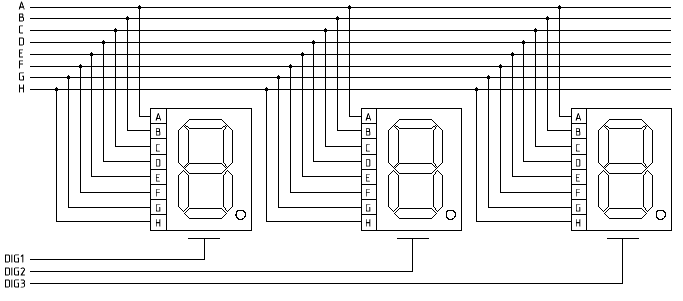
\includegraphics[width=0.7\textwidth]{158_Indi.png}
\caption{Динамическая индикация}
\end{figure}

% Вопрос 159 ----------------------------------------------------------
\section{Загрузчики. Процедура загрузки. Статические и динамические загрузки.}

Загрузчик операционной системы --- системное программное обеспечение, обеспечивающее загрузку операционной системы непосредственно после включения компьютера.

Загрузчик операционной системы:

\begin{itemize}
\item обеспечивает необходимые средства для диалога с пользователем компьютера (например, загрузчик позволяет выбрать операционную систему для загрузки);
\item приводит аппаратуру компьютера в состояние, необходимое для старта ядра операционной системы (например, на не-x86 архитектурах перед запуском ядра загрузчик должен правильно настроить виртуальную память);
\item загружает ядро операционной системы в ОЗУ. Загрузка ядра операционной системы не обязательно происходит с жесткого диска. Загрузчик может получать ядро по сети. Ядро может храниться в ПЗУ или загружаться через последовательные интерфейсы (это может пригодиться на ранней стадии отладки создаваемой компьютерной системы);
\item формирует параметры, передаваемые ядру операционной системы (например, ядру Linux передаются параметры, указывающие способ подключения корневой файловой системы);
\item передаёт управление ядру операционной системы. 
\end{itemize}

При работе с реальной памятью распределять ресурсы возможно двумя путями:

\begin{itemize}
\item Назначить для каждой задачи объем памяти фиксированного размера;
\item Деление памяти на переменные фрагменты: размер каждого фрагмента, отведенного памяти под задачу определяется требуемым объемом памяти.
\end{itemize}

Как результат второй подход экономит память --- нет «свободных хвостиков».

Причем память можем делить в статике --- до начала первого вычисления, либо же динамически распределять память --- приходит задача, возьмите пустой раздел. При статическом делении первоначально программа определяет требуемые фрагменты для выделения в памяти и только после этого назначает адреса для каждой задачи. Если задача требует памяти больше чем имеющийся фрагмент, задание не может быть загружено и оно ожидает очереди.

Основная проблема при загрузке заданий в выделенные фрагменты --- коррекция адресов прямых ссылок. Все такие адреса можно модифицировать согласно начальному адресу, выделенного фрагмента в памяти.

Статистический способ --- не самый оптимальный по результатам работы процессора. Часто простаиваем. Поэтому используем динамическую загрузку, какая либо из задач завершена на ее место в память можно загрузить следующую задачу из очереди и запустить на выполнение. При этом другие находятся на счете. Если объем новой задачи превышает освободившийся объем в памяти, возникают трудности. При загрузке в разделы фиксированного объема, как правило, имеющаяся память устраивает любые задачи --- в крайнем случае, можно подождать второй освободившийся фрагмент и загружать сразу 2. Когда же работаем с сегментами переменной длины загружать большое задание приходиться в 2 свободного фрагмента.
В этом случае проще сформировать один целый фрагмент памяти, в который и загрузить новую задачу.

Когда при выполнении текущего задания образуется свободное адресное пространство, появляется шанс загрузить в это свободное пространство новую задачу.

Но задача лежит на диске. Поэтому режим ПДП и «подгрузка» требуемых данных в основную память --- slooping --- перемещение всего фрагмента --- задания с диска в память и обратно. Перемещением с жесткого диска в память занимается программа, называемая загрузчик. Соответственно загрузчики бывают: абсолютные и относительные (перемещающие). Абсолютные --- по фиксированным адресам; относительные --- по изменяющимся по времени адресам фрагмента памяти, выделенных заданием. Соответственно загрузка может проводиться статическая --- до начала работы и в процессе работы --- динамическая.


% Вопрос 160 ----------------------------------------------------------
\section{Управление реальной памятью. Виртуальная память. Таблица соответствия адресов.}

В многопрограммном режиме работы возникает задача размещения загружаемых программ в ОЗУ.  Участки памяти, куда загружаются программы, определяются с помощью программы управления памятью --- диспетчера памяти. В зависимости от сложности задачи выделяют несколько стратегий управления памятью:

\textit{Статическое деление} --- разделение памяти на участки фиксированного объема, обычно применяется в простейших случаях (2-3 программы). Если процессов много, часть из них должна ожидать своей очереди для размещения в памяти, пока не завершатся предыдущие загруженные программы. Загрузка программы возможна только в том случае, если объем раздела в памяти больше объема программы, следовательно с такой системой загрузки всегда остается неиспользуемое свободное место в памяти, что снижает эффективность ее использования.

\textit{По запросу} --- деление памяти на фрагменты переменной длины. Процессы стоящие в очереди получают необходимый для загрузки объем памяти, следовательно память используется эффективнее. Когда один или несколько процессов завершатся, в освободившуюся область памяти загружаются новые процессы из очереди, которые однако имеют другой размер, поэтому в занимаемой памяти образуются <<дыры>>. Чтобы исправить эту проблему производится \textit{дефрагментация} --- сдвиг одного из массивов к окончанию другого. При этом возникает задача нахождения в кодах абсолютных ссылок и изменения их, для их нахождения команды переходов по абсолютным адресам могут быть отмечены специальным битом (технически это не предусмотрено в системе команд) либо при компиляции в конец файла могут быть записаны адреса таких команд. Для выполнения дефрагментации требуется специальная программа для пересылки массивов.

Другая проблема возникает, когда работающий процесс затребовал дополнительную память, поэтому массив новых данных формируется в другом сегменте памяти. В таком случае программа управления памятью работает как редактор связей: делает ссылку в текущих кодах на новое адресное пространство.

Загрузку программ в память выполняет загрузчик, который выполняет пересылку по необходимым адресам. Загрузка в память выполняется по параграфам (младшая тетрада адреса загрузки равна нулю). Загрузка может производиться в статическом (сначала загружаются все задачи, затем выполняются), либо в динамическом (в промежутках между работой загружаются другие задачи) режимах.

Основная память ВС ограничена, в то же время используя ВЗУ можно попеременно по одним и тем же адресам в основной памяти загружать коды из внешней памяти и работать с ними. Такую организацию памяти называют \textit{виртуальной}. Основная проблема при таком алгоритме работы --- связывание конкретной задачи с адресами в ВЗУ. Кроме того, при работе с файлам может возникнуть необходимость сохранения их в ВЗУ, для этого используется таблица соответствия адресов.

\begin{figure}[H]
\centering
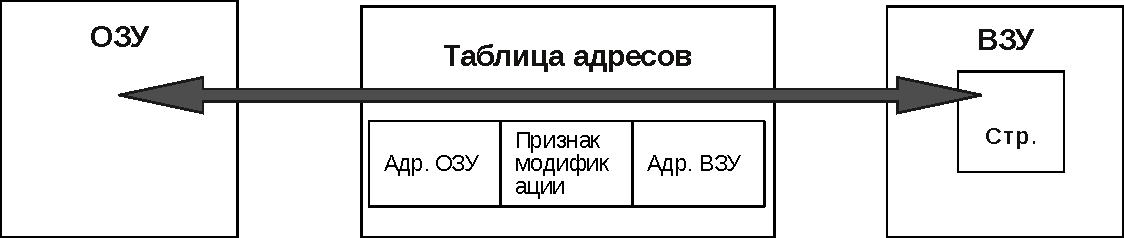
\includegraphics[width=0.7\textwidth]{160_virtual_memory.pdf}
\caption{Схема работы с виртуальной памятью}
\end{figure}

\end{document}